\documentclass[dvisvgm,multi=true]{standalone}
\usepackage{mathmlcoresvg}
\begin{document}
%<figcaption><span>Figure 21: </span>Box model for the <code>msup</code> element</figcaption>
  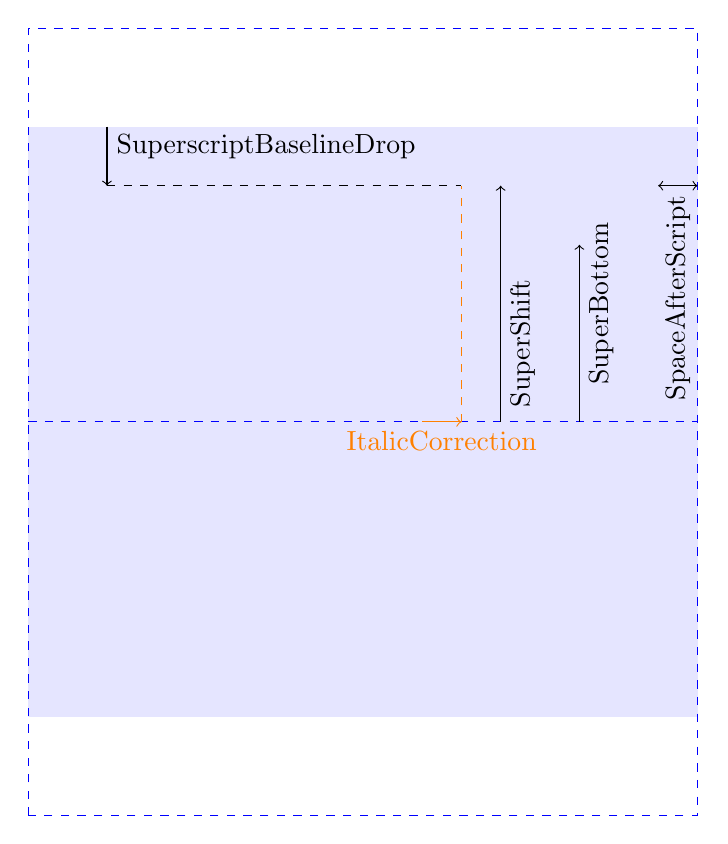
\begin{tikzpicture}[yscale=-1]

  \fill[blue!10](0,3.75) rectangle (8.5,-3.75);

  \MathMLBox{0}{0}{1}{2.5}{red};

  \MathMLBox{5.5}{-3}{.5}{.5}{green};

  \draw[dashed,blue](0,5) rectangle(8.5,-5)
  (0,0)--(8.5,0);

  \draw[->] (6,0) -- (6,-1)node[below,rotate=90]{SuperShift} -- (6,-3);

  \draw[orange,->] (5,0) --
   (5.25,0)node[below]{ItalicCorrection} -- (5.5,0);
  \draw[dashed,orange] (5.5,0)--(5.5,-3);

  \draw[->] (7,0) -- (7,-1.5)node[below,rotate=90]{SuperBottom} -- (7,-2.25);

  \draw[<->] (8,-3) -- (8.25,-3)node[left,rotate=90]{SpaceAfterScript} -- (8.5,-3);

  \draw[->] (1,-3.75) -- (1,-3.5)node[right]{SuperscriptBaselineDrop} -- (1,-3);
  \draw[dashed] (1,-3) -- (5.5,-3);
\end{tikzpicture}

\end{document}
